\section{Methodology}
\label{sec:Meth}

Architecture of our method can be divided into 
4 modules, as shown in
Figure~\ref{fig:netStruct}. 
Image Feature Extractor, 
which contains three pretrained models of 
DenseNet, which are trained on ImageNet task 
is used as the backbone of our network structure. 
Benefited from pre-trained models, the network 
gains the ability to extract basic features 
from images before training. 
Designing three different models has aimed for 
diverse features. 
To make use of different representation power 
of each model, fusing the feature from each 
model with weight add method.
Hash Decoder, wherein the image object 
is randomly divided into a plurality of 
branches, each bit corresponds to a hash. 
By this step, the model can not only improve 
the generalization ability of the model, and 
may simplify the calculation of high-dimensional 
features, to facilitate the work of the 
classifier.
Using the third module for classification, 
we also used three classifiers, including 
SVM (Support Vector Machine), KNN (K Nearest 
Neighbor) and RF (Random Forest).
This design of classifications is to help 
improve the accuracy of model predictions.
The fourth module is a linear regression 
analysis model, which has been utilied the 
RPN(Region Proposal Network) proposed by 
Faster RCNN. 
To do this, it is aimed at marking the specific 
location of the lesion in mammography.

\subsection{Network design}
\label{sec:MethNet}

Hand-crafted features have been widely used in 
the mammography image classification tasks. 
While feature-based approach these handmade 
perform well, they are always too complicated 
to build and constraints may under certain 
circumstances.
With the development of deep learning, deep 
convolutional neural networks can extract 
intricate features from raw data
\cite{Szegedy2016,Zeiler2014}.
After AlexNet great success in ImageNet 
competition, the potential of deep 
CNNs are gradually discovered by researchers, 
many deep network architectures with good 
performance on image classification tasks 
such as VGGNet, GoogLeNet, ResNet, DenseNet 
and etc, network based on these well-performed
architectures are naturally applied to 
mammography image recognition task. 
We build a fusion network made of four 
modules which are feature extractor(Explained 
in detail in 
Section~\ref{sec:MethNetFea}), 
hash decoder(Explained in detail in 
Section~\ref{sec:MethNetHash}),
classifier(Explained in detail in 
Section~\ref{sec:MethNetCls}) 
and regression model(Explained in detail in 
Section~\ref{sec:MethNetReg}). 

\subsubsection{Feature Extractor Module}
\label{sec:MethNetFea}

In the modules, building it with a truncated 
DenseNet without the fully connected layers
\cite{Huang2017}. 
The backbone of DenseNet consists of 3 dense 
blocks, each ciphertext block is composed 
of several compact layers. 
The number of dense layers in each dense block 
increases while the dense blocks go deeper.
Dense block structure is shown in 
Figure~\ref{fig:DenseBlock}.

\begin{figure*}[!ht]
    \centering
    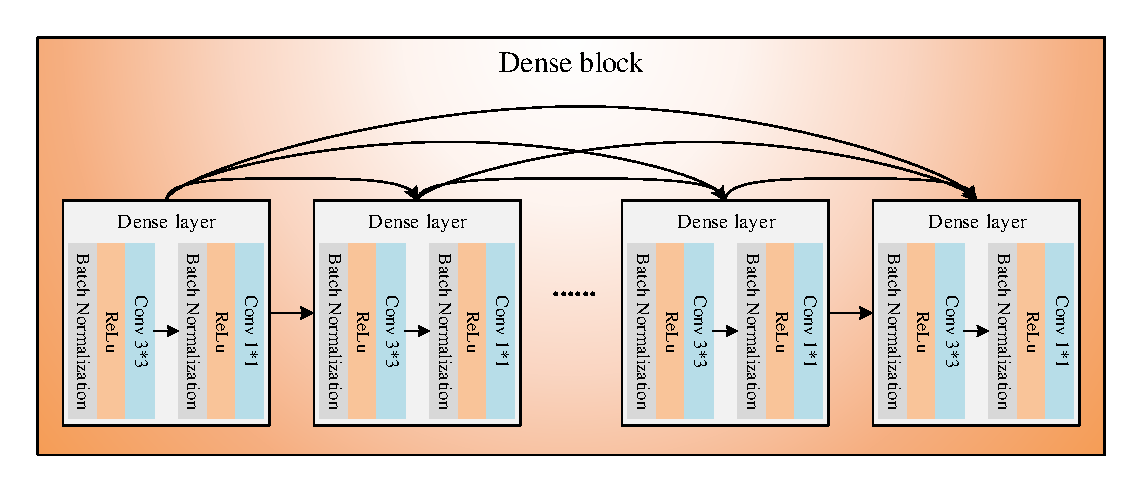
\includegraphics[
        width=0.78\textwidth,
        keepaspectratio
    ]{DenseBlock.pdf}
    \caption{The architecture of DenseNet.}
    \label{fig:DenseBlock}
\end{figure*} 

As DenseNet, different from the normal output 
of each dense layer are fed to all subsequent 
dense layer in the same block are connected 
through intensive, this is achieved by 
operating in series.
By this way, from beginning to end global 
information may traverse dense blocks, each a 
dense layer may obtain additional knowledge 
from previous knowledge.
For a dense layer, which comprises a base 
layer 2, the base layer of each batch 
normalized by layer, and two RELU activation 
function convolution layers.
\cite{Srivastava2014,Ioffe2015,Kingma2015}. 
Further, a feature extractor to help 
positioning the input feature the most 
abundant block portion, and a transitional 
layer and a batch standardization convolution 
layers, followed by the largest pool layers, 
which are inserted into each two between 
dense blocks.
It is set for down sampling the output feature 
maps of each dense block. 
With the development of the network, the 
magnitude of the output characteristics of figure 
decreases, while the number of dimensions will 
increase the output characteristic of figure
\cite{Huang2017}.
An example of the output feature maps after 
each dense block is shown in 
Figure~\ref{fig:imgFea}.

\begin{figure*}[!ht]
    \centering
    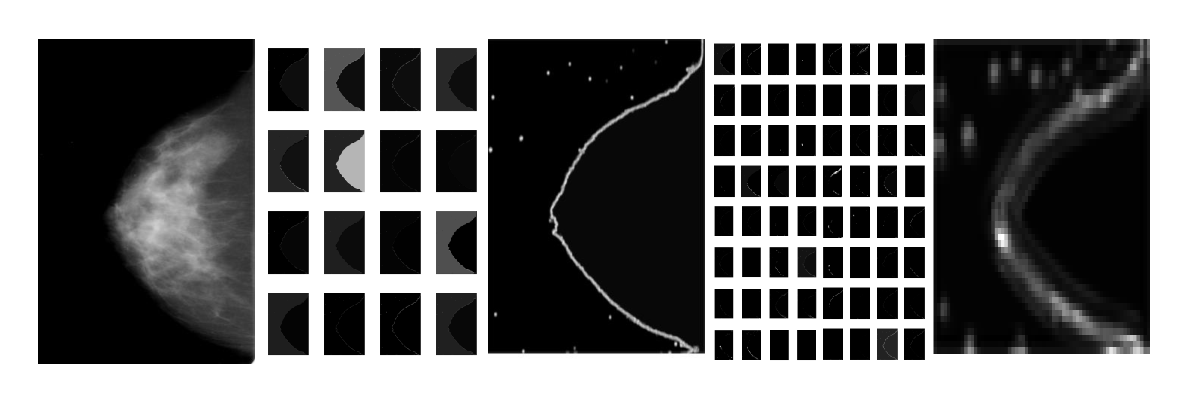
\includegraphics[
        width=1.0\textwidth,
        keepaspectratio
    ]{ImgFea.pdf}
    \caption{The feature of the 
        fusion of extractors' result.}
    \label{fig:imgFea}
\end{figure*} 

Usually, most CNN based methods on mammography 
image classification tasks use a single network 
to extract features. 
However, we found some work by different ways to 
complete this work.
It attempts to explore the potential of fusion 
of features extracted from different models. 
Wherein the fusion tag in two models with 
predictive input image, based on a AlexNet, on 
the other GoogleNet. 
Compared with the single network method, it 
utilizes different functions with higher 
precision.
Inspired this proposed a method has the same 
structure by fusing, through a number of 
different models of transfer of learning 
strategy training to improve classification 
accuracy.
Note shallow layer tends to extract the basic 
characteristics, the deeper layer tends to 
abstract feature extraction, leading to the 
conclusion, the fixed parameters model 
different layers having different features will 
focus on the complexity of the training phase.
\cite{Ciresan2012}.
In the inference phase, the model will be 
trained together to take advantage of the 
different features of each model extraction 
capability.

Different from it, train 3 models with 
the same structure, but freeze different 
layers of each model while training 
concurrently. There are two reasons why we 
select 3 same DenseNet based model to be fused. 
Firstly, we have tested the single-model 
method for this task, among which DenseNet
performs best. Secondly, we have tried fusing 
different trained models such as Inception, 
ResNet, DenseNet structures together with frozen 
parameters, fusing 3 DenseNet based models 
is still the better way. We think the reason 
is that when fusing models in different 
topological structures, the relationship 
between features extracted from 3 models is 
relatively weak and we cannot assure that 
they are learning different knowledge from 
training images. Since the structures of 
different networks varies greatly, models may
concentrate on similar features with different 
performance according to the depth of network. 
By training 4 similar structure models with 
different frozen layers, each model extracts 
features in different levels based on the 
number of frozen parameters, we can ensure 
that every model concentrates on different 
features of the input image. Meanwhile, in
the experiment we found the false positive 
and false negative instances of each model 
are quite different, which proves that they 
are concentrating on different kinds of 
features. Since the 3 models keep a similar 
network structure, Their relationship 
extracted features stronger, and better 
integration features.

\begin{figure*}[!ht]
    \centering
    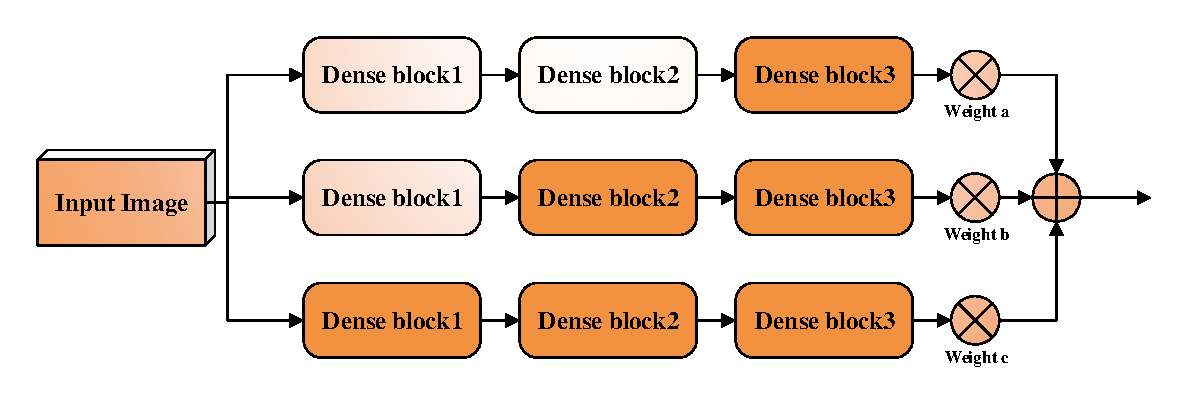
\includegraphics[
        width=0.78\textwidth,
        keepaspectratio
    ]{ExtractorFusion.pdf}
    \caption{The module of feature through such steps, the model can not 
    only improve the generalization ability of the 
    model, but also simplify the calculation of 
    high-dimensional features to facilitate the work 
    of the classifier extractors' fusion.}
    \label{fig:extrFusion}
\end{figure*} 

As figure~\ref{fig:extrFusion}
shows, training 3 models with parameters in 
different block frozen in parallel. 
Each row represents one model, the dense block 
in bright means that the parameters in this 
block are frozen during the training phase 
while the dark block means that parameters 
are activated.
we fuse the feature of multiple transfer 
learning models with a weighted sum operation. 
The weights of 3 models are set manually in 
the experiments. 
With the advantages of functional diversity, 
the transfer learning mode fusion method 
achieves high accuracy in mammography 
image recognition tasks.


\subsubsection{Hash Decoder Module}
\label{sec:MethNetHash}

After obtaining the intermediate image 
features from feature extractor module, 
we propose a hash decoder module, the map 
image features to the hash code.
As seen in the Figure~\ref{fig:hashDecoder}, 
the proposed hash decoder module first randomly 
divides the feature vector into several slices 
of equal length\cite{Lai2015}.
Each slice is then connected by a full layer, 
then, is in the range [0,1] to the output limit 
value of the activation function s-shaped, and 
the threshold function is mapped to a segment 
of a size to encourage bit output binary hash.
After that, connect the output hash bits as a
code.
A hashing decoder module may be a simple 
alternative to complete the connection layer, 
wherein the layer of the intermediate image 
mapped to the input vector, the vectors then 
converted to the activation function.
Compared with this choice, the key idea of the 
overall strategy is to try to reduce redundancy 
between the hash bits.
Several recent studies have advocated the use 
of the hash code has fewer redundant bits.

\begin{figure*}[!ht]
    \centering
    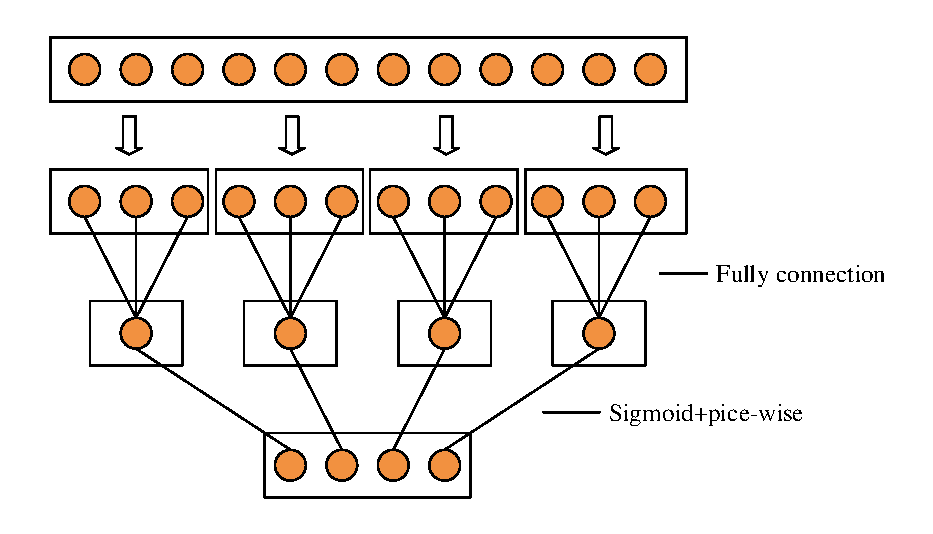
\includegraphics[
        width=0.66\textwidth,
        keepaspectratio
    ]{HashDecode.pdf}
    \caption{The module of the hash decoder.}
    \label{fig:hashDecoder}
\end{figure*} 

To encourage hash decoder output binary code, 
we used activation function, then the 
fragmentation threshold function.
Given a 50-dimensional slice 
$x^{(i)}(i=1,2,...q)$
, 50 pairs of output is defined as a fully 
connected layers

\begin{equation}
    \label{eq:eq_descr_1}
    fc_i(x^{(i)}) = W_ix^{(i)}
\end{equation}

with $W_i$ being the weight matrix.

Given $c=fc_i(x^{(i)})$, the sigmoid function
is defined by 

\begin{equation}
    \label{eq:eq_descr_2}
    sigmoid(c) = \frac{1}{1+e^{-\beta c}}
\end{equation}

where $\beta$ is a hyper-parameter.

The piece-wise threshold function is to 
encourage binary outputs. Specifically, for an 
input variable $s = sigmoid(c) \in [0,1]$, 
this piece-wise function is defined by

\begin{equation}
    \label{eq:eq_descr_3}
    y = \left\{
        \begin{array}{lr}
            0, & s < 0.5-\epsilon \\
            s, & 0.5-\epsilon \le 0.5+\epsilon \\
            1, & s > 0.5+\epsilon
        \end{array}
    \right.\nonumber,
\end{equation}

where $\epsilon$ is a small positive 
hyper-parameter.

This fragmentation threshold function similar 
to a hard-coded behavior, and encourages the 
use of binary output in the training. 
Specifically, if the outputs from the sigmoid 
function are in $[0, 0.5-\epsilon]$ or 
$[0.5+\epsilon, 1]$, they are truncated to be 
0 or 1, respectively. Note that in prediction, 
the proposed deep architecture only generates 
approximate (real-value) hash codes for input 
images, where these approximate codes are 
converted to binary codes by quantization. 
With the proposed piece-wise threshold 
function, some of the values in the 
approximate hash codes are already zeros or 
ones. Hence, less errors may be introduced
by the quantization step.

\subsubsection{Classifier Module}
\label{sec:MethNetCls}

In the classifier module, building it with
a fusion structure by SVM, KNN, Random
Forest classic methods. For each method, it 
predicates with the output of the hash decoder,
then the three results weight add, as the 
result of class information. There is a reason
why we select 3 different classifiers to be 
fused. These three algorithms target 
different classification types, so the 
results obtained for different feature 
information will also be different. The 
biggest advantage of doing this is to 
improve the robustness of the model, 
and at the same time it also improves 
the accuracy of model recognition. 

\begin{figure*}[!ht]
    \centering
    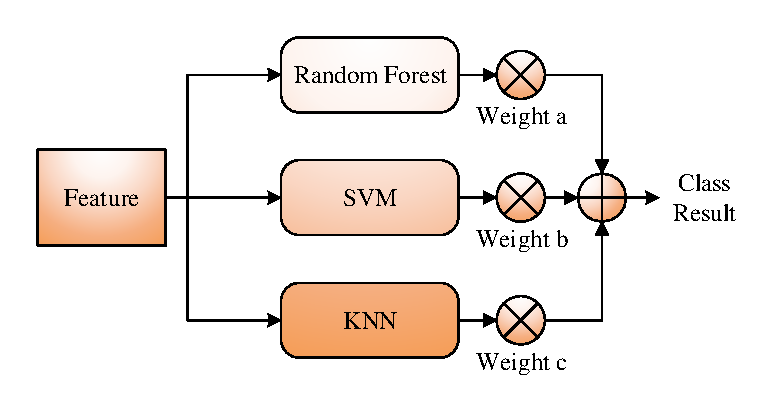
\includegraphics[
        width=0.58\textwidth,
        keepaspectratio
    ]{ClassifierFusion.pdf}
    \caption{The module of the fusion of 
        classifier.}
    \label{fig:classifierFusion}
\end{figure*}   

\subsubsection{Regression module}
\label{sec:MethNetReg}

Proposed area network (the RPN) receiving 
(any size) image as an input, and outputs a 
set of rectangular objects proposed are each 
offer it has an objective rating.
To generate the proposed region, a slide on 
a small network last layer output shared.
The network is fully connected to the input 
of the conversion characteristics of FIG 
n × n window space.
Each sliding window is mapped to a low 
dimensional vectors.
This vector is fed into two fully connected 
layers at the box regression 
layer and the box classification layer.
As shown in Figure~\ref{fig:RPN}

\begin{figure*}[!ht]
    \centering
    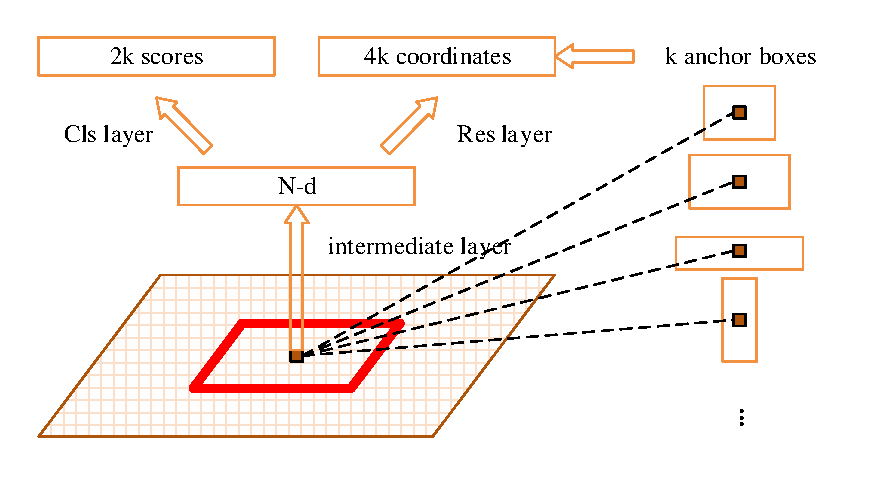
\includegraphics[
        width=0.68\textwidth,
        keepaspectratio
    ]{RPN.pdf}
    \caption{The module of the region proposal 
        network.}
    \label{fig:RPN}
\end{figure*} 


Note that, since the small network operated 
sliding window, the whole connection layer at 
all spatial positions shared. 
The architecture is naturally implemented with 
the n×n CONV layer followed by two brothers 
1×1 CONV layer\cite{Ren2017}.
And the loss function is defined by

\begin{equation}
    \label{eq:eq_descr_4}
    L({p_i},{t_i})=\frac{1}{N_{cls}}\sum_iL_{cls}(p_i,p_i^*)
     + \lambda\frac{1}{N_{reg}}\sum_ip_i^*L_{reg}(t_i,t_i^*)
\end{equation}

In order to perform regression, we use the 
following 4 coordinate parameterization::

\begin{eqnarray}\label{eq:eq_descr_5}
    t_x=(x-x_a)/w_a, 
    t_y=(y-y_a)/h_a, 
    t_w=log(w/w_a), 
    t_h=log(h/h_a), \\
    t_x^*=(x^*-x^*_a)/w_a, 
    t_y^*=(y^*-y^*_a)/h_a, 
    t_w^*=log(w^*/w_a), 
    t_h^*=log(h^*/h_a)
\end{eqnarray}

This can be thought of as 
bounding-box regression from an anchor box 
to a nearby ground-truth box.

\subsection{Transfer learning}
\label{sec:MethTL}

Aims to transfer learning between the source 
and target domains related to knowledge 
transfer, which is a useful tool for machine 
learning, can have a positive impact on the 
field due to insufficient training data and 
difficult to apply.
Transfer learning methods can be divided into 
four categories: case-based, based on the 
mapping, network-based, learning against 
depth migration
\cite{Pan2010,Tan2018}.
Most network-based approach used in the 
convolution neural network.
It is achieved by transferring the network 
structure and pre-trained parameters of the 
source domain into a part of a deep 
convolutional neural network used in the 
target domain. 
In our work, we constructed a feature 
extractor according to the following in 
Section~\ref{sec:MethNetFea}, 
then we initialize the network parameters 
with the parameters of a DenseNet model 
that were pre-trained on the ImageNet dataset.

In our experiments, adjusting the size of 
the input image to one piece, going that 
dataset; 
freezing, which consists of leaving the 
parameters in shallow part of the 
pretrained model unchanged and training 
only the rest part of the network, which can 
make use of the basic feature extracting 
ability of pretrained model. Freezing layers 
or not in training phase depends on the 
number of category and quantity variance 
between source and target dataset. 
Compared to other datasets, the DDSM 
dataset we used are much smaller. 
Moreover, most images in both datasets 
are natural images, they are similar in 
a way, hence we freeze some of the layers 
during training. In order to explore the 
effect of fusing different feature extractors, 
we try different freezing strategy on the 
networks, the details are described in 
Section~\ref{sec:MethNetFea}. 
